%!TEX root = avollmer.tex

\section{Supplementary Information \\ \todo{not included in the icdl paper}

\section{Introduction}
Recent research on robot learning in the field of developmental robotics has begun to take into account the feedback of a human tutor in social interaction \cite{breazeal2004tutelage}. Let's consider the overall goal of developing a robot system which should learn from and interact with non-expert users. Without assuming that the robot understands human feedback (i.e., without programming the information on how and when feedback is given into the robot system beforehand) how should the system understand what the signals it perceives mean and what they are referring to (cf. Gavagai problem \cite{quine1960word})? % additional motivation? 

In interaction, humans align and effortlessly, maybe even automatically, create common ground in communication \cite{clark1991grounding,pickering2004toward}. However, unlike humans who assume an immense amount of shared information, a robot system cannot rely on already established protocols for interacting. This is because, on the one hand, little is known about the universal interaction protocols humans rely on in communication and on the other hand, human-robot interaction (HRI) is still very different from human-human interaction, as it is clearly characterized by asymmetry and restrictedness in the sense that the human and the robot in general do not have the same abilities, modalities, mechanisms, and body for communication, perception and action \cite{lohse2010investigating}. For example, a robot that does not have arms cannot gesture, a robot without the respective algorithms or sensors does not perceive gaze direction or understand speech commands, and without any knowledge of internal computational mechanisms it is difficult to assess how a robot perceives its interaction partner and his/her actions. It is thus important that robots are able to negotiate meaning online with their interaction partners.

We designed an experimental setup with which we aim at investigating the processes used by humans to negotiate a protocol of interaction used to solve a collaborative task, when they do not already share one. In the current paper, we present and justify the method used and mention the very first preliminary results obtained from a pilot study employing the setup. This research undertaking should inform us about what are the main issues in building robots capable of similar interactional flexibility. We are for instance interested in what kind of strategies humans use to align and what kind of meanings of social signals they converge to. Whereas, on the long run, the obtained findings could be used as priors for a robotic system interacting with humans, in an initial step, we first need to shed light on how interaction protocols are negotiated in \emph{restricted, asymmetric human-human interaction}. To our knowledge, there exists little research in the field of linguistics or pragmatics on this topic. To investigate this process of negotiation, we chose to design an experimental semiotics study which enables us to modify communication in the desired way, namely to restrict communication between participants who are assuming asymmetric roles. The field of experimental semiotics studies the emergence and evolution of communication systems \cite{galantucci2009experimental}. Here, instead of computer simulations as conducted by others (see \cite{cangelosi2002simulating,steels2012experiments}), controlled experiments in laboratory settings are designed to observe communication between participants who perform joint tasks. For instance, Galantucci et al. showed that pairs of participants performing a joint task could coordinate their behavior by agreeing on a symbol system \cite{galantucci2005experimental}.


In our study, two people play a game in restricted, asymmetric communication conditions. For the task in the game, the communication between participants should be indispensable. Thus, it should not be solvable by either one of the participants alone, e.g. with mere exploration. Therefore, we designed the task to be a joint construction task with asymmetric roles: the role of a builder and the role of an architect. With building blocks, the builder should assemble a target structure which is unknown to him/her but which the architect knows. 
Communication is not face-to-face but restricted, so that it is not possible for participants to communicate via familiar verbal or non-verbal communication channels, as for example speech or gestures. At the same time, the setup does not constrain all aspects of communication and thereby preserves a certain degree of naturalness in communication. It gives participants much freedom with respect to some features, including timing and rhythm or possible meanings (e.g. of button presses). The setup does not impose a predefined sequence of interaction upon participants, as it is often done in HRI scenarios \cite{akgun12hri}, but still benefits from a laboratory setting in which we do not need to take the full complexity of natural social interaction into account. With the aim to simulate sending feedback to an interaction partner who does not have the same perceptual capabilities -- similar as in an interaction with a robot --, in our study the architect does not know how exactly his/her feedback is perceived by the builder. For the successful completion of the thus highly challenging joint task of the game, both participants have to learn how to interact with each other. Thus, failing to complete the game successfully is equivalent to failing to communicate successfully.


The main contribution of the current paper is the presentation of the novel experimental method of our study. We would like to demonstrate that it allows to study important questions for the understanding of human negotiation of interaction protocols in joint construction tasks and that these questions are very important for HRI in the long-term. Also, we report preliminary results of a first pilot run of the study. We first briefly discuss related work, then present our method and the preliminary results of the pilot study and close with a conclusion.



\subsection{Meanings}

\textbf{Meaning switches and reset} During the experiment, we noticed some participants were misinterpreting a \emph{Positive feedback} as a \emph{Negative feedback} (and reversely), but most of the time they were able to detect and correct this misunderstanding. In few cases, it was the architect that inverted the meaning of the signals but in most cases it was the builder that had to reinterpret the signals, often after a \emph{Reset} instruction from the architect. The data we collected are not detailed enough for a fine-grained temporal analysis but we are able to count the number of feedback interpretation switches per run. In 5 out of 14 successful games (see Figure~\ref{fig:feedback_switch_enhanced}) the architect or the builder changed his use or interpretation of signals between positive and negative feedback.

\begin{figure}[!ht]
  \begin{center}
      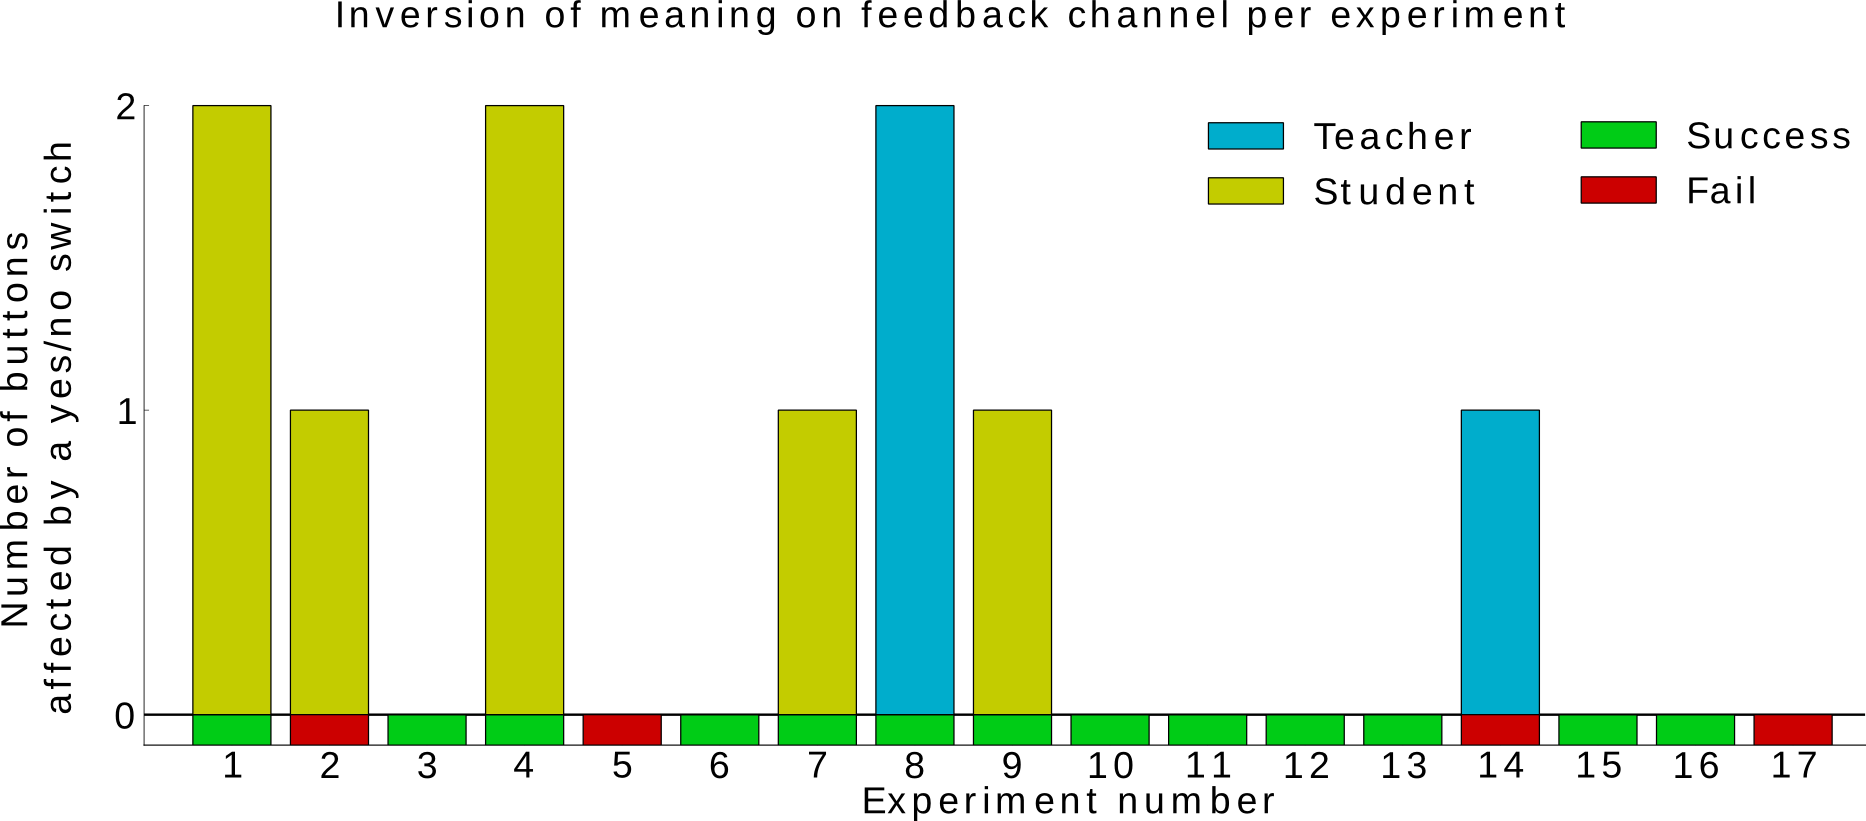
\includegraphics[width=\columnwidth]{media/plots/inversion_meaning}
      \caption{Number of signals whose meanings switch between positive and negative feedback during the experiment. In blue, cases where the architect decides to change the meaning of a button from one feedback type to the other. In yellow, cases where the builder changes his/her interpretation of a signal. The colored bar on the bottom indicates if the experiment was successful or not.}
    \label{fig:feedback_switch_enhanced}
    \end{center}
\end{figure}

\textbf{Context dependent meaning} In several cases the architect pressed all buttons to signify a salient event. This event was either perceived as a \emph{Reset} instruction if the builder felt lost or an \emph{End} instruction if the builder felt confident about his/her understanding of the previous interaction sequences. This is illustrated in figure~\ref{fig:timeline}, where at $t=200 s$, as players already tried for several iteration with no success, the architect presses all buttons to signify a \emph{Reset}. After this \emph{Reset}, a new set of symbols is used by the architect which is well understood. Finally, to signify that the construction is finished, the architect presses again all buttons simultaneously now with the intended meaning that the task is completed. As the interaction was going well, this signal was understood as a \emph{End} signal by the builder and the experiment goes to a successful end.

Taking a closer look at the failed experiments, we find that in one of them, where the builder presented one block at a time, in the end the target construction was almost finished. Architect and builder understood each other, but what happened is that an early mistake in the position of one block was not signalled and thus corrected by the architect right away. He waited until the rest of the structure was completed and then tried to address the mistake by means of the introduction of a new signal. This new signal was interpreted by the builder as an \emph{End} feedback, leading to the end of the game with one block in a position next to the target one. With respect to the other failed experiments, the structure at the time the game ended was far from the target construction and there was no noticeable progress in all three cases.



\textbf{Timing} Figure~\ref{fig:timeline} can be analyse at the global scale but also at a very local one, it contains information on which feedback the architect gives to the builder at which points in time aligned with the construction progress. 

\textbf{Confirmation bias} Some builders were affected by the so called confirmation bias. While mistaking negative feedback for positive they were going quite far in a wrong direction, even if the signal would seem contradictory for an outside observer. It was very difficult for them to re-assess their belief, they better thought the architect was mistaking or were pursuing in a very improbable direction. I think no students were able to overcome the confirmation bias problem by themselves, leading either to a failed experiment or needed the architect to produce a salient event to reset the experiment. With the recorded data, it is unfortunately not possible to quantify this phenomenon even if the figure~\ref{fig:feedback_switch_enhanced} gives a good first intuition.

\subsection{Builder Strategies}

\textbf{Workspace} From the videos, we observed that many participants in the role of the builder (7 out of 17) cleaned their workspace in the beginning of the experiment, so no block is present anymore, and tried to maintain a clean workspace during the game. A clean workspace gave them a presentation space, where they could propose blocks in an unambiguous way. Two builders additionally started out with a clean workspace, but one did not remove incorrect blocks he proposed and thus did not maintain the clean workspace and the other moved all blocks in the workspace at one point in the game. Another strategy was pursued by eight builders who from the beginning kept all blocks on the workspace and therewith enabled the architect to witness the process of choice of block. Of these eight builders, three neatly ordered and aligned their blocks on the workspace and proposed one block at a time by pointing to it. The remaining five builders did not order or align the blocks in any way. These participants opened up a workspace inside the overall workspace (i.e., proposing blocks in-between or next to the rest).
\begin{itemize}
\item clean workspace used as presentation space (9)
\item all blocks in view (8) (nicely aligned (3), or not aligned (5))
\end{itemize}

\textbf{Propositions} Essentially the task consisted in two subtasks, finding correct blocks and joining them. For this, participants proposed blocks and positions of blocks in different ways. For proposing blocks in search for a correct one, builders ``present'' blocks by placing them alone on the workspace or in a separate sub-workspace, they point to the block they wish to receive feedback about, or they lift the respective block to highlight it.
\begin{itemize}
\item present
\item point
\item lift
\end{itemize}
To find at which position a specific block is correctly joined with others, the propositions differ in the level of accuracy and precision of the proposed position. Some builders begin with bumping two blocks together to receive feedback about if they should be joined at all. In some cases the respective block is placed above, below, on the right or on the left of a structure to receive course feedback about the location of the correct position. Another way of presentation is to continuously move the respective block around the structure with expected positive feedback when the correct position is reached. Some builders discretely test or propose positions on the way around the structure by only pausing, joining blocks half way, or fully joining the blocks at each possible position.
\begin{itemize}
\item bump
\item order (bottom to top)
\item right, left, above, below
\item continuously move around the structure
\item discretely stop at each position or join half-way
\item join at each possible position
\end{itemize}

